% SWINQ: one sensor, one forehand, in 3D  -- Beamer pitch (3 minutes)
% Compile with pdflatex (Overleaf: upload this folder, compiler pdfLaTeX).
% Transitions/animations show in full-screen PDF viewers (Adobe Reader, Okular, Evince).
% Speaker notes: uncomment the pgfpages line to get notes on a second screen.
\documentclass[aspectratio=169,11pt]{beamer}
\usepackage[T1]{fontenc}
\usepackage[utf8]{inputenc}
\usepackage{lmodern}
\usepackage{amsmath,amssymb}
\usepackage{textcomp}
\usepackage{tikz}
\usetikzlibrary{arrows.meta,positioning,shapes.geometric,calc,shadows}
% \usepackage{pgfpages}\setbeameroption{show notes on second screen=right}

% ---------- colours: Tampere University purple + accents ----------
\definecolor{tauPurple}{HTML}{4E008E}
\definecolor{tauDeep}{HTML}{2B0050}
\definecolor{tauLilac}{HTML}{B79CD9}
\definecolor{tauMist}{HTML}{F3EEF9}
\definecolor{accGold}{HTML}{FFB81C}
\definecolor{accOrange}{HTML}{FF8C00}
\definecolor{accGreen}{HTML}{2EB82E}
\definecolor{inkGrey}{HTML}{4A4458}

\usetheme{default}
\setbeamertemplate{navigation symbols}{}
\setbeamercolor{background canvas}{bg=white}
\setbeamercolor{normal text}{fg=tauDeep}
\setbeamercolor{frametitle}{fg=white,bg=tauPurple}
\setbeamercolor{structure}{fg=tauPurple}
\setbeamercolor{alerted text}{fg=accOrange}
\setbeamercolor{block title}{fg=white,bg=tauPurple}
\setbeamercolor{block body}{fg=tauDeep,bg=tauMist}
\setbeamertemplate{itemize item}{\color{accGold}\scriptsize$\blacksquare$}
\setbeamertemplate{blocks}[rounded][shadow=false]
\setbeamerfont{frametitle}{size=\Large,series=\bfseries}
\setbeamertemplate{frametitle}{%
  \nointerlineskip
  \begin{beamercolorbox}[wd=\paperwidth,ht=2.4em,dp=0.9em,leftskip=1.2em]{frametitle}
    \usebeamerfont{frametitle}\insertframetitle
  \end{beamercolorbox}%
  \vspace{-0.15em}{\color{accGold}\rule{\paperwidth}{2pt}}}
\setbeamertemplate{footline}{%
  \hfill{\color{tauLilac}\scriptsize SWINQ $\cdot$ Hack For Humanity\quad\insertframenumber/\inserttotalframenumber\quad}\vspace{0.6em}}

% big-number helper
\newcommand{\bignum}[2]{\begin{minipage}[t]{\linewidth}\centering
  {\fontsize{30}{32}\selectfont\bfseries\color{tauPurple}#1}\\[0.3em]{\small\color{inkGrey}#2}\end{minipage}}
\newcommand{\deg}{\ensuremath{^{\circ}}}

\title{One sensor. One forehand. In 3D.}
\subtitle{Rebuilding a tennis swing from the SWINQ dampener}
\date{Hack For Humanity $\cdot$ Sports Telemetry}

\begin{document}

% ================= 1. Cover =================
{\setbeamercolor{background canvas}{bg=tauPurple}
\begin{frame}[plain]
\transfade[duration=0.6]
\begin{tikzpicture}[remember picture,overlay]
  \fill[tauDeep] (current page.south west) rectangle ([yshift=1.1cm]current page.south east);
  \fill[accGold] ([yshift=1.1cm]current page.south west) rectangle ([yshift=1.18cm]current page.south east);
  \foreach \r/\o in {3.2/0.10,2.4/0.14,1.6/0.18}
    \draw[white,opacity=\o,line width=6pt] ([xshift=-2.2cm,yshift=-1.0cm]current page.north east) circle (\r);
\end{tikzpicture}
\begin{columns}[c]
\column{0.5\textwidth}
  {\color{accGold}\small\bfseries SWINQ $\cdot$ HACK FOR HUMANITY}\\[0.6em]
  {\color{white}\fontsize{30}{33}\selectfont\bfseries One sensor.\\One forehand.\\In 3D.}\\[0.8em]
  {\color{tauLilac}\small A full swing rebuilt from the small sensor\\on the strings: no cameras, no mocap suit.}
\column{0.5\textwidth}
  \uncover<2->{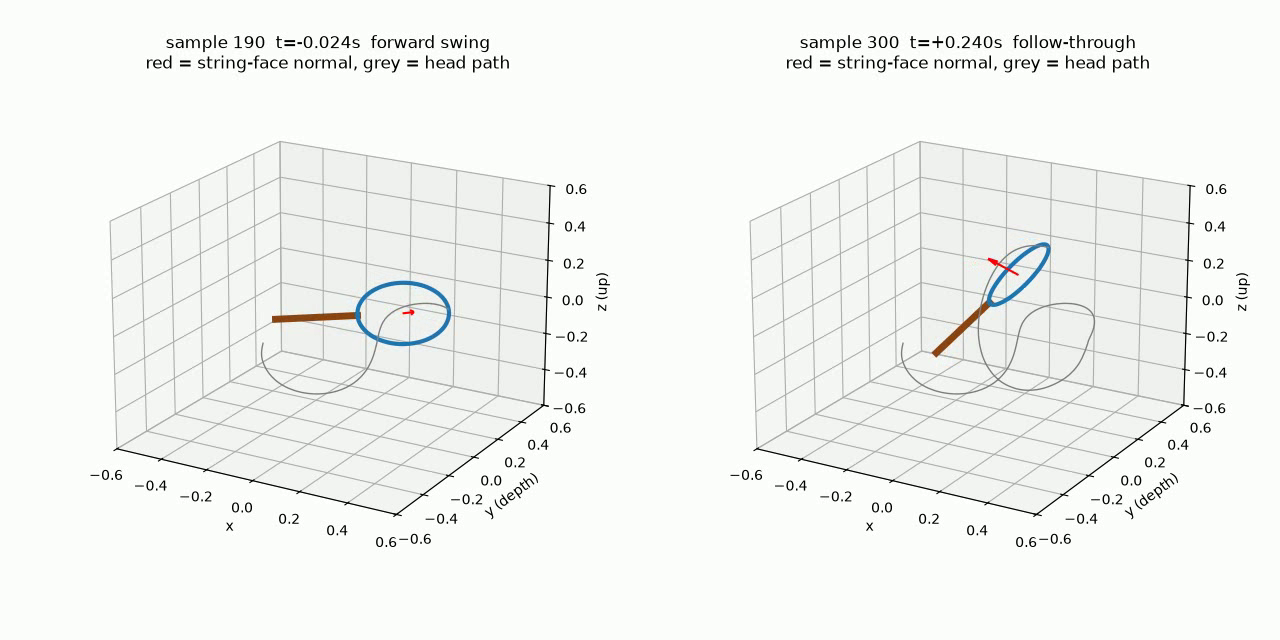
\includegraphics[width=\linewidth]{img/stroke_frames.png}}
\end{columns}
\note{[0:00--0:20] SAY: This is one tennis forehand, rebuilt in 3D using only the small sensor clipped onto the strings. No cameras, no special suit. One tiny sensor, recording for less than a second.
PLAIN WORDS: the sensor is like the motion sensor in your phone. Brown = handle, blue = head, red arrow = way the strings face, grey = path of the head.}
\end{frame}}

% ================= 2. The challenge =================
\begin{frame}{The data is hard}
\transdissolve[duration=0.5]
\vspace{0.8em}
\begin{columns}[t]
\column{0.32\textwidth}\uncover<1->{\bignum{0.96\,s}{400 readings, 416 per second.\\Starts mid-swing: never still.}}
\column{0.32\textwidth}\uncover<2->{\bignum{1720\deg/s}{peak spin: almost\\5 full turns per second}}
\column{0.32\textwidth}\uncover<3->{\bignum{16\,g}{force sensor maxes out\\for 18 readings before impact}}
\end{columns}
\vspace{1.4em}
\uncover<3->{\begin{center}
\begin{tikzpicture}
  % sketch: a clipped signal
  \draw[->,inkGrey] (0,0) -- (8,0) node[right]{\scriptsize time};
  \draw[->,inkGrey] (0,0) -- (0,1.6) node[above]{\scriptsize force};
  \draw[dashed,accOrange] (0,1.0) -- (7.6,1.0) node[right]{\scriptsize 16\,g limit};
  \draw[very thick,tauPurple] plot[smooth] coordinates {(0,0.1) (1.5,0.2) (3,0.45) (4,0.8) (4.4,1.0)};
  \draw[very thick,tauPurple] (4.4,1.0) -- (5.6,1.0);
  \draw[very thick,tauLilac,dashed] plot[smooth] coordinates {(4.4,1.0) (5.0,1.45) (5.6,1.9)};
  \node[accOrange,font=\scriptsize] at (5.0,0.65) {sensor reads ``max''};
\end{tikzpicture}\end{center}}
\note{[0:20--0:45] SAY: The data is tough. Less than one second, starting mid-swing, so we never see the racket still. It spins at over 1,700 degrees per second, and just before impact the force sensor maxes out.
PLAIN WORDS: to know which way is up you normally hold the sensor still and feel gravity; here it is never still. 16 g limit is like a bathroom scale that stops at 100 kg.}
\end{frame}

% ================= 3. How it works =================
\begin{frame}{How it works}
\transpush[direction=0]
\begin{center}
\begin{tikzpicture}[
  box/.style={rounded corners=6pt,draw=none,fill=#1,text=white,minimum height=1.05cm,
              text width=2.55cm,align=center,font=\small\bfseries,drop shadow},
  arr/.style={-{Stealth[length=3mm]},very thick,tauLilac},
  node distance=0.55cm]
  \node[box=tauPurple] (s) {Sensor\\spin + force};
  \node[box=tauPurple,right=of s] (i) {Add up the\\small turns};
  \node[box=tauDeep,right=of i] (o) {Racket angle\\every 2.4\,ms};
  \node[box=accGold,text=tauDeep,right=of o] (b) {3D model\\(Blender)};
  \draw[arr] (s) -- (i); \draw[arr] (i) -- (o); \draw[arr] (o) -- (b);
  \uncover<3->{\node[box=inkGrey,below=0.9cm of i] (v) {Two videos\\(referee)};
  \draw[arr,accGold] (v) -- node[left,font=\scriptsize,text=inkGrey]{start angle} (i);
  \draw[arr,accGold,dashed] (v) -| node[below,pos=0.25,font=\scriptsize,text=inkGrey]{check + correct} (o);}
\end{tikzpicture}
\end{center}
\vspace{-0.2em}
\begin{columns}[t]
\column{0.48\textwidth}
\uncover<1->{\begin{block}{1. Turning $\rightarrow$ angle}
\[\underbrace{\theta_{\text{new}}}_{\text{angle now}} = \underbrace{\theta_{\text{old}}}_{\text{angle before}} + \underbrace{\omega\,\Delta t}_{\text{small turn}}\]
\small Done 416$\times$ per second, in full 3D (quaternions). Tested: 0.03\deg{} error.
\end{block}}
\column{0.48\textwidth}
\uncover<2->{\begin{block}{2. Physics fills the gap}
\[a = \omega^{2}\, r \qquad (r = 0.65\,\text{m})\]
\small Faster spin $\Rightarrow$ harder outward pull. Spin is known, so the missing force can be filled in.
\end{block}}
\end{columns}
\note{[0:45--1:20] SAY: Three things. The sensor tells us how fast the racket turns; adding up those small turns gives its angle. Where the force sensor maxed out, physics fills the gap: spin speed tells us how hard it pulled. And two videos act as a referee.
PLAIN WORDS: like counting your turns with eyes closed. Like a car in a corner: faster = pushed out harder. Like a step counter, the sensor knows changes, not the start, so the start angle comes from video.}
\end{frame}

% ================= 4. Numbers =================
{\setbeamercolor{background canvas}{bg=tauDeep}
\setbeamercolor{normal text}{fg=white}
\begin{frame}{What the sensor tells a player}
\transfade[duration=0.5]
\vspace{0.4em}
\begin{columns}[t]
\column{0.5\textwidth}
\uncover<1->{{\fontsize{34}{36}\selectfont\bfseries\color{accGold}89 km/h}\\[0.2em]
{\small\color{tauLilac} racket-head speed at impact}\\[0.2em]
{\small $v = \omega\,r = 26.7\,\tfrac{\text{rad}}{\text{s}}\times 0.92\,\text{m} \approx 24.6\,\tfrac{\text{m}}{\text{s}}$}}\\[1.0em]
\uncover<2->{{\fontsize{34}{36}\selectfont\bfseries\color{accGold}85\deg}\\[0.2em]
{\small\color{tauLilac} racket turn in the last 0.1\,s before impact}}
\column{0.5\textwidth}
\uncover<3->{{\fontsize{34}{36}\selectfont\bfseries\color{accGold}$\approx$30\,g}\\[0.2em]
{\small\color{tauLilac} true peak force, above the 16\,g limit}}\\[1.0em]
\uncover<4->{{\fontsize{34}{36}\selectfont\bfseries\color{accGold}581\,Hz}\\[0.2em]
{\small\color{tauLilac} string vibration (likely)}\\[0.2em]
{\small $f_{\text{true}} = 416 \pm 165\ \Rightarrow\ 251$ or $581$\,Hz}}
\end{columns}
\note{[1:20--1:45] SAY: From the sensor alone: the racket head moved at about 89 km/h at impact, it turned 85 degrees in the last tenth of a second, the real force peaked near 30 g, and the strings rang at about 580 vibrations per second. Say 89 km/h slowly.
PLAIN WORDS: speed = how fast it turns times how far the head is from the wrist. The sensor reads too slowly to see the strings directly, like wagon wheels in films that seem to spin backwards, so we work backwards.}
\end{frame}}

% ================= 5. Check against cameras =================
\begin{frame}{Checked against two cameras}
\transdissolve[duration=0.5]
{\small Green = racket from the sensor alone. Top: front camera. Bottom: rear camera. Left $\rightarrow$ right: time.}\\[0.5em]
\begin{tikzpicture}
  \node[inner sep=0] (img) {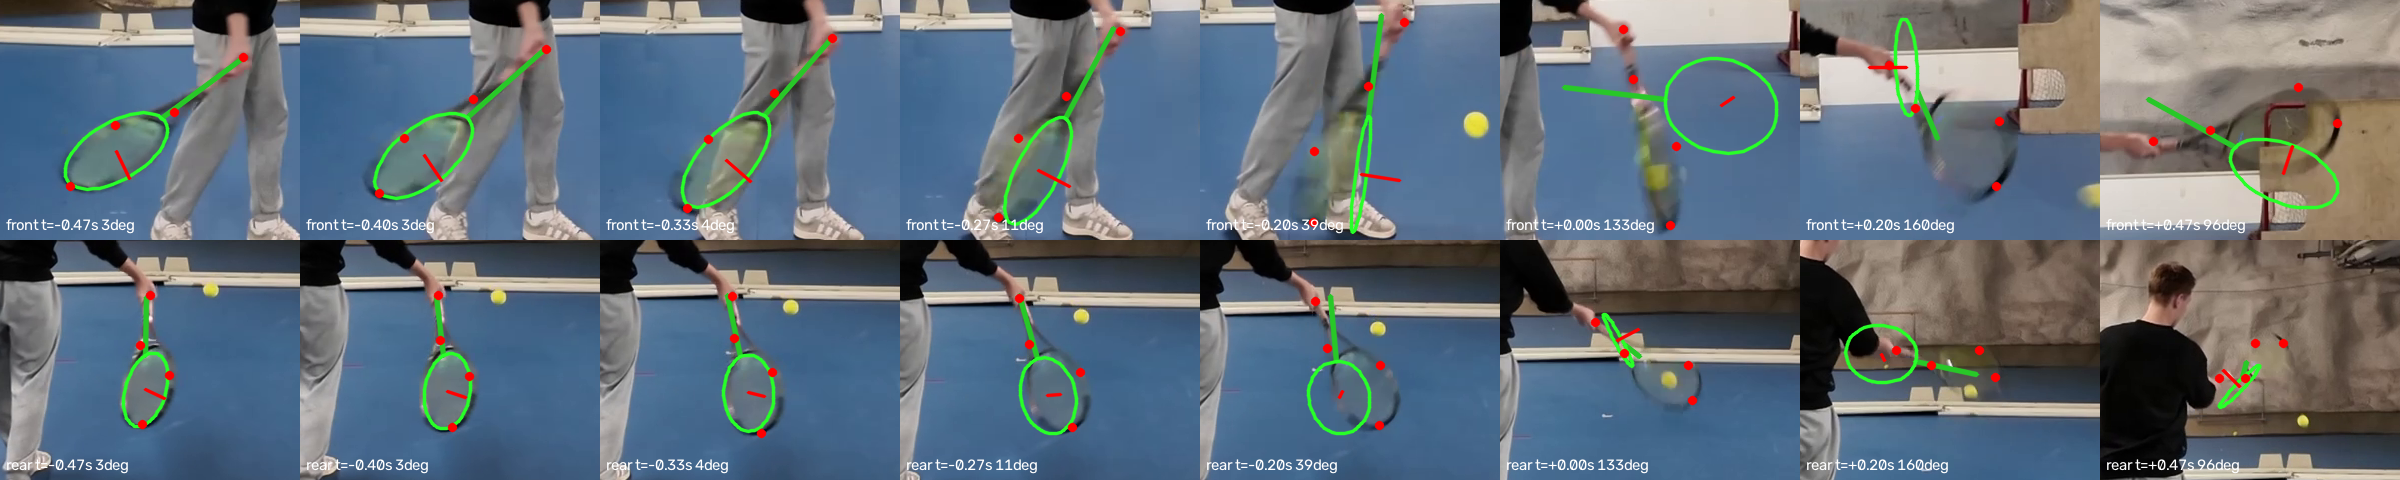
\includegraphics[width=\textwidth]{img/contact_sensor_only.png}};
  \uncover<2->{\draw[accGreen,line width=2pt,rounded corners] ($(img.south west)+(0.02,0.02)$) rectangle ($(img.south west)!0.5!(img.north west)+(0.5\textwidth,0)+(0,0.0)$);}
  \uncover<2->{\draw[accGreen,line width=2pt,rounded corners] (img.north west) rectangle ($(img.north west)+(0.5\textwidth,-\paperheight*0)+(0,-0.01)$);}
\end{tikzpicture}\\[0.6em]
\only<2>{\textcolor{accGreen}{\bfseries Early swing: within 11\deg.}}%
\only<3->{\textcolor{accOrange}{\bfseries Fast part of the swing: it drifts}\ (gyro sees 2--3$\times$ more turn than the 30\,fps video).}
\note{[1:45--2:10] SAY: To check our work we used two videos. Green is our sensor's racket drawn on the real footage. Early in the swing it matches; as the swing speeds up it drifts.
PLAIN WORDS: small counting mistakes add up. Best explanation: blurry 30 fps video and camera/sensor clocks not perfectly lined up. We ruled out axis set-up, recording speed and mounting angle.}
\end{frame}

% ================= 6. GP correction =================
\begin{frame}{Correcting the drift}
\transpush[direction=90]
\begin{columns}[c]
\column{0.42\textwidth}
\uncover<1->{\begin{block}{Idea}
\small At each video frame, measure the error $e_i$.\\Draw a smooth curve $\hat e(t)$ through the errors (Gaussian process), then remove it:
\[q_{\text{corrected}}(t) = q_{\text{sensor}}(t)\cdot \exp\!\big(\hat e(t)\big)\]
\end{block}}
\uncover<2->{\begin{center}
{\fontsize{30}{32}\selectfont\bfseries\color{inkGrey}88\deg}
\begin{tikzpicture}[baseline=-0.6ex]\draw[-{Stealth[length=3mm]},line width=3pt,tauPurple] (0,0) -- (1.1,0);\end{tikzpicture}
{\fontsize{30}{32}\selectfont\bfseries\color{tauPurple}12.4\deg}\\[0.2em]
{\scriptsize\color{inkGrey} mean error, tested on frames the correction never saw}
\end{center}}
\column{0.56\textwidth}
\uncover<3->{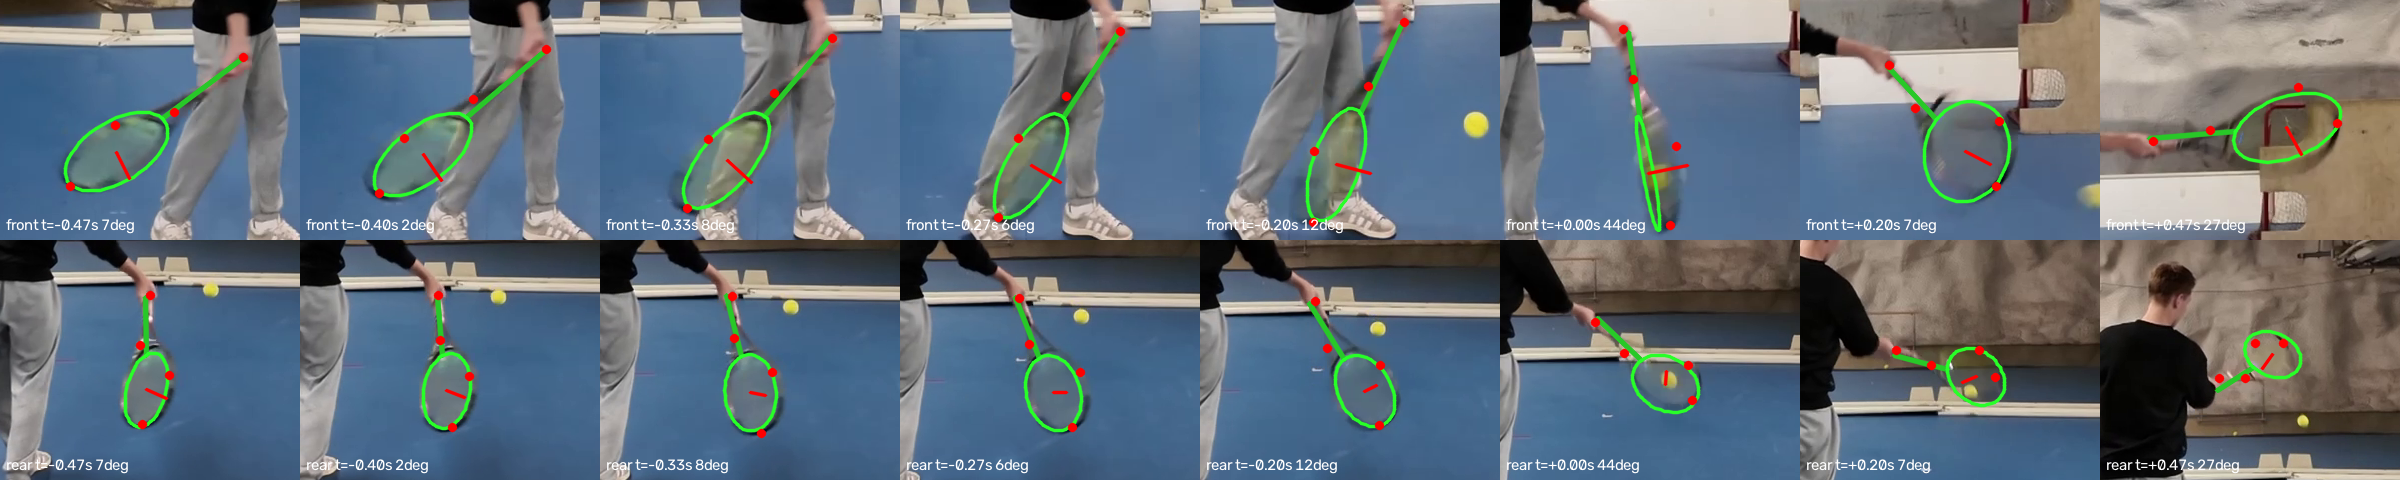
\includegraphics[width=\linewidth]{img/contact_gp.png}\\[0.3em]
{\scriptsize\color{inkGrey} Corrected racket (green) now follows the real racket through impact. Play \texttt{gp\_correction.mp4}: orange = before, green = after.}}
\end{columns}
\note{[2:10--2:45] SAY: So we correct the drift. At every video frame we measure how far off we are, draw a smooth curve through those errors and remove it. Tested fairly, on frames it never saw, the error drops from 88 to about 12 degrees.
PLAIN WORDS: like checkpoints in a race with a smooth curve between them. We hid one frame at a time and predicted it. The corrected racket combines sensor + video; the numbers on slide 4 are sensor-only.}
\end{frame}

% ================= 7. Close =================
{\setbeamercolor{background canvas}{bg=tauPurple}
\setbeamercolor{normal text}{fg=white}
\begin{frame}[plain]
\transfade[duration=0.8]
\begin{tikzpicture}[remember picture,overlay]
  \fill[tauDeep] (current page.south west) rectangle ([yshift=1.1cm]current page.south east);
  \fill[accGold] ([yshift=1.1cm]current page.south west) rectangle ([yshift=1.18cm]current page.south east);
\end{tikzpicture}
\vspace{1em}
{\fontsize{22}{26}\selectfont\bfseries Open, tested, ready to extend}\\[1.2em]
\begin{columns}[t]
\column{0.31\textwidth}\uncover<1->{{\color{accGold}\bfseries Python package}\\{\small\color{tauLilac}one script per stage, 18 tests}}
\column{0.31\textwidth}\uncover<2->{{\color{accGold}\bfseries orientation.csv}\\{\small\color{tauLilac}racket angle for every reading}}
\column{0.31\textwidth}\uncover<3->{{\color{accGold}\bfseries Blender script}\\{\small\color{tauLilac}builds and animates the racket}}
\end{columns}
\vspace{2em}
\uncover<4->{{\fontsize{20}{24}\selectfont\bfseries\color{accGold} Motion capture from a tennis dampener.}\\[0.4em]{\color{white}Thank you!}}
\note{[2:45--3:00] SAY: Everything is open and tested and runs from one small sensor. Knowing the racket's angle at every moment is the hardest half of full motion tracking. Motion capture from a tennis dampener. Thank you.}
\end{frame}}

\end{document}
